%% LaTeX2e class for student theses
%% sections/evaluation.tex
%% 
%% Karlsruhe Institute of Technology
%% Institute for Program Structures and Data Organization
%% Chair for Software Design and Quality (SDQ)
%%
%% Dr.-Ing. Erik Burger
%% burger@kit.edu
%%
%% Version 1.3, 2016-12-29

\chapter{Evaluation}
\label{ch:Evaluation}

This chapter is structured as follows: Initially the concept is elaborated (\autoref{sec:Evaluation:concept}), followed by evaluation scenarios (\autoref{sec:Evaluation:scenarios}) and the evaluation of the single tasks: monitoring (\autoref{sec:Evaluation:monitoring}), privacy analysis (\autoref{sec:Evaluation:monitoring}), model generation (\autoref{sec:Evaluation:privacyanalysis}), adaptation planning (\autoref{sec:Evaluation:planning}) and finally adaptation execution (\autoref{sec:Evaluation:execution}).

\section{Evaluation Design}
\label{sec:Evaluation:concept}

iObserve Privacy is a complex approach with many depending tasks. Evaluating the program as a whole is next to impossible due to the multiplexing dependencies. The evaluation factors would not be manageable and inconclusive results would make the evaluation itself pointless. So we decided to evaluate every task independently. The order and structure got inspired by the iObserve pipeline.

%Accuracy => Scenarios => unbiased
The task evaluation is generally split into an \textit{Accuracy} evaluation and a \textit{Scalability} evaluation. The accuracy evaluation aims for the correct functionality, testing whether the actual results are conform to expected results. For the evaluation we are creating a set of \textit{Evaluation Scenarios}, which reflect real world situations by defining a staring point and an expected endpoint. If the systems result differs from the endpoint, the reasons must be found and analysed.

%Scalability => Runtime behaviour, automatic generated PCMs, 1 > 10 > 100 > 1000 ... logarithmic scale
The scalability evaluation aims for the systems runtime characteristic, based on an increasing work load. The actual accuracy result of the task doesn't interest during this analysis. The primary measurement is the task response time, dependent on the assembly context count and resource container count. Both axis are logarithmic scaled, so the response behaviour is clearly visible. The individual models are randomly generated, based on a repository model input.

\section{Evaluation Scenarios}
\label{sec:Evaluation:scenarios}

The scenarios are structured in \textit{PRE}, \textit{EVENT}, \textit{REACTION} and \textit{POST}. Pre describes the distributed software system before the event takes place. The event is a trigger for a certain process or task chain, usually referenced as reaction. Post defines the state of the software system after the reaction.

The scenarios describe the behaviour of iObserve Privacy through all tasks, while each task gets evaluated individually. Nevertheless, details of an scenario may need clarification during the evaluation of this task.

The scenarios are derived from \cite{Heinrich.2016b}. This paper describes potential runtime changes to a distributed software system. However, not all mentioned scenarios are of interest in the privacy analysis context. Scenarios 1 and 2 represent the observed system runtime changes. However, major iOberve privacy failing scenarios are not covered. This is due to the iObserve Privacy design specific nature of error states. Scenario 3 and 4 cover these error.

\subsection{Scenario 1: Default}
\label{eval:scenario:1}
% PRE: Amazon Deployment @ EU WEST
% CASE: Critical Error => Amazon moves instances to EU WEST & US EAST
% POST: Migration Monitored, Privacy Analysis started
%					=> IF OK:	Do nothing 
%					=> IF BAD:	Calculate Alternative (Privacy Compliant) => Plan => Adapt => Evaluate!
This scenario describes the "default" setting. A migration gets monitored, analysed, an alternative deployment calculated and finally migrated. The process works completely automated. This means no operator interaction is required and no task error is generated. As trigger for privacy analysis the server geo-location migration is used.
\begin{itemize}
	\setlength\itemsep{0em}
	\item \textbf{PRE}: All components of the software system are deployed on Amazons EC2 service on the \textit{EU Frankfurt} location. The system is privacy compliant.
	\item \textbf{EVENT}: Amazons EU Frankfurt data centre has a critical failure. As a result Amazon starts migrating local virtual machines towards the US Ohio and EU Ireland locations.
	\item \textbf{REACTION}: iObserve Privacy monitors the migration and starts a privacy analysis. If the analysis doesn't show a privacy violation no further action is taken. If the analysis shows a privacy violation, an alternative, privacy compliant deployment gets computed, a system adaptation plan gets calculated and finally executed.
	\item \textbf{POST}: The software system is in a privacy compliant state.
\end{itemize}


\subsection{Scenario 2: System extension}
\label{eval:scenario:2}
% PRE: 	Privacy components @ Microsoft; Non-Privacy @ UKRAINE
% CASE:	New DePersonalized Component gets deployed @ UKRAINE
% POST: Deployment Monitored => Privacy Analysis started => "Joining Data Streams" found => Calculate Alternative (Privacy Compliant) => Plan => Adapt => Evaluate!

This scenario describes the deployment runtime change. The deployment of a new software component triggers a privacy analysis, which detects "joining data streams" (see \autoref{sec:PrivacyAnalysis:theory}). This triggers the generation of an alternative deployment and the system adaptation. The pipeline works like in Scenario 1 without any operator interaction.
\begin{itemize}
	\setlength\itemsep{0em}
	\item \textbf{PRE}: All personal categorized components of the software system are deployed on Amazons EC2 service on the \textit{EU Frankfurt} location. All other components are hosted by an Ukrainian provider. The system is privacy compliant.
	\item \textbf{EVENT}: The system operator adds another as depersonalised categorized component to the Ukrainian host.
	\item \textbf{REACTION}: iObserve Privacy monitors the migration and starts a privacy analysis. The privacy analysis shows a privacy violation due to joining data streams. An alternative, privacy compliant deployment gets computed, a system adaptation plan gets calculated and finally executed.
	\item \textbf{POST}: The software system is in a privacy compliant state.
\end{itemize}

\subsection{Scenario 3: Failing Adaptation}
\label{eval:scenario:3}
% PRE: 	All @ Cheap Hoster (Europe SLA)
% CASE:	Some components migrate @ UKRAINE
% POST: Deployment Monitored => Privacy Analysis started => Privacy Violation found => Calculate Alternative (Privacy Compliant) => Plan => Adapt can't be done automatically => Call the Operator
This scenario describes the operator-in-the-loop use case, when an adaptation sequence can't be executed automatically. The migration of a software component results in a privacy violating state. After the generation of a privacy compliant alternative and the calculation of the adaptation sequence, the operator is required. One or more adaptation actions can't be executed automatically. This is usually due to missing source control, like the \textit{Change Repository Component Action} or the \textit{Allocation Action}.
\begin{itemize}
	\setlength\itemsep{0em}
	\item \textbf{PRE}: All components of the software system are hosted multiple server instances by cloud reseller. 
	\item \textbf{EVENT}: The reseller starts migrating his server to another cloud providers.
	\item \textbf{REACTION}: iObserve Privacy monitors the migration and starts a privacy analysis. The privacy analysis shows a privacy violation. An alternative, privacy compliant deployment gets computed. The adaptation calculation shows certain steps can't be executed automatically. After ordering the adaptation steps the operator gets informed for manual execution.
	\item \textbf{POST}: iObserve Privacy shows the operator the adaptation sequence with emphasis on the manual tasks.
\end{itemize}


\subsection{Scenario 4: Missing Alternative}
\label{eval:scenario:4}
% PRE: 	All @ Cheap Hoster (Europe SLA)
% CASE:	Some components migrate @ UKRAINE
% POST: Deployment Monitored => Privacy Analysis started => Privacy Violation found => Calculate Alternative (Privacy Compliant) => No Privacy Compliant Alternative Found => Call Operator
This scenario describes the use case, where no privacy compliant, alternative deployment could be calculated. The migration of a software components results in a privacy violating state. The calculation of privacy compliant alternatives deployment fails. The operator needs to be informed about the current situation.
\begin{itemize}
	\setlength\itemsep{0em}
	\item \textbf{PRE}: All components of the software system are hosted multiple server instances by cloud reseller. 
	\item \textbf{EVENT}: The reseller starts migrating his server to another cloud providers.
	\item \textbf{REACTION}: iObserve Privacy monitors the migration and starts a privacy analysis. The privacy analysis shows a privacy violation. An alternative, privacy compliant deployment can't be computed.
	\item \textbf{POST}: \dots
	\todo{Specify end state!}
\end{itemize}

%\subsection{Scenario 5}
% PRE: 	Privacy components @ Amazone EU WEST; Non-Privacy @ Cheap Hoster (Europe SLA)
% CASE:	Cheap Hoster constantly migrates to the cheapest hoster => Moves two Depersonal instances to the same server in Ukraine
% POST: Migration Monitored, Privacy Analysis started
%			=> "Joining Data Streams" found => Calculate Alternative (Privacy Compliant) => Plan => Adapt => Evaluate!

\subsection{Futile Scenario}
There are a couple of scenarios which don't apply to iObserve Privacy, due to various reasons \cite{Heinrich.2016b}. We will elaborate those scenarios shortly.

%Performance
Performance or workload characteristics are not tackled, since performance and privacy analysis combined wouldn't be manageable in the scope of this thesis.

%Undeployment
The un-deployment or de-replication are two scenarios which reduce the complexity of the privacy analysis. A privacy violation can't be triggered by eliminating a component and/or a server from the system.

%Replication
The replication of a server, with all its components, will trigger a deployment event. This means, this scenario is already covered by \textit{Scenario 2}.


\section{Evaluation Models}
\label{sec:Evaluation:models}

In the previous sections we defined a couple of scenarios for the evaluation. In order to execute these scenarios, we need PCM Privacy models (\autoref{ch:pcmExtension}). Scenario and model need to get selected individually, depending on task to evaluate.

\subsection{CoCOME-Cloud}
\label{sec:eval:models:cocome}

The \textit{CoCOME Cloud} PCM model is a representation of the CoCOME system as a distributed cloud variant. It is a representation of a supermarket IT infrastructure. It exists of six individual deployed components:  \textit{logic.webservice.cashdeskline.cashdeskservice}, \textit{Cloud.Web}, \textit{traidingsystem.inventory}, \textit{traidingsystem.cashdeskline}, \textit{webservice.inventory} and \textit{traidingsystem.external.bank}. The system is oriented on real systems with dozens of interfaces and multiple composite components. As a result, CoCOME-Cloud is very complex and not suited for the evaluation of specific aspects. However, it is as the only available model fully specified and "PerOpteryx ready". See \cite{Heinrich.2015} for detailed information on CoCOME.


\subsection{Medi System}
\label{sec:eval:models:medSys}

\begin{figure}[h]
	\centering
	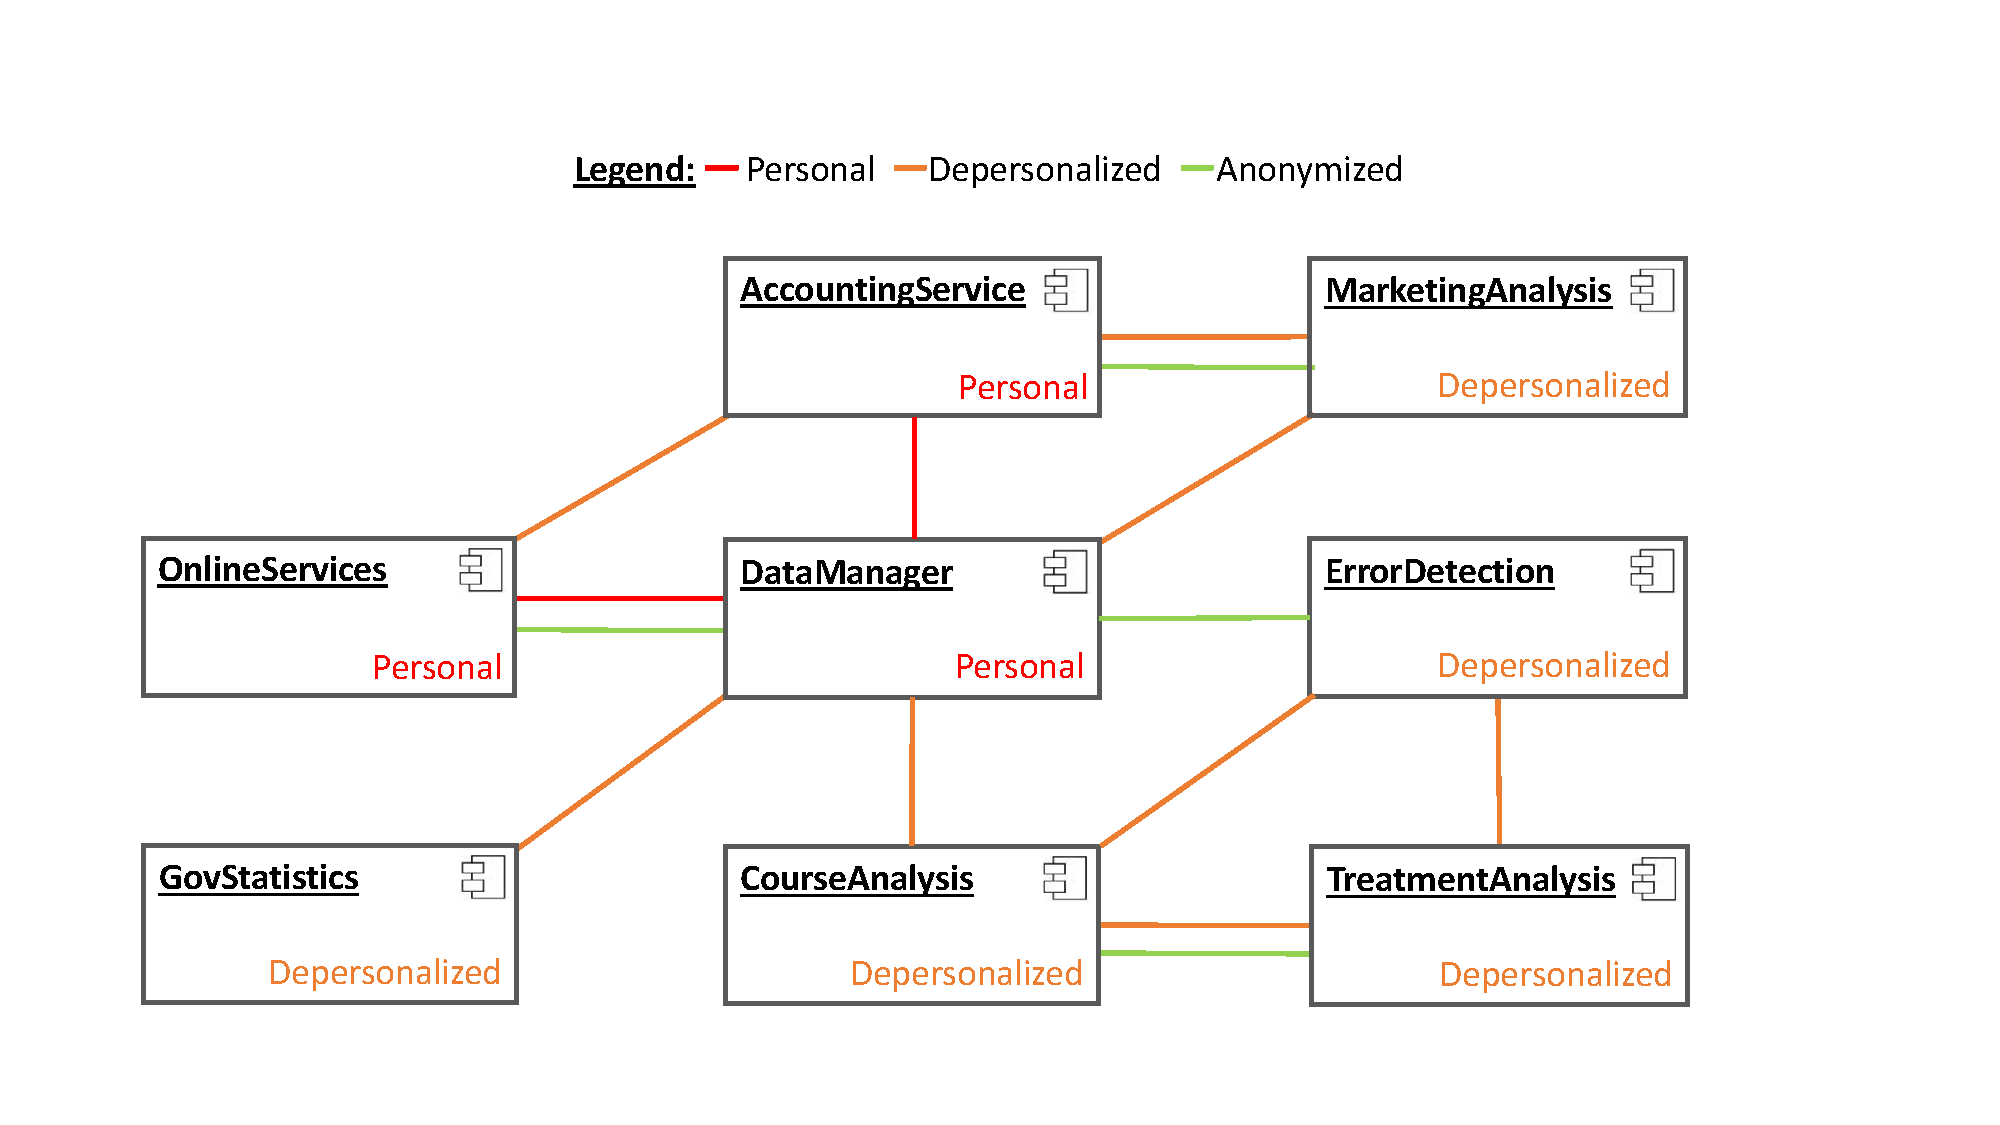
\includegraphics[trim = 0mm 10mm 0mm 20mm, clip, width=0.90\textwidth]{graphs/medSystem_noserver}
	\caption{Initial component categorization}
	\label{fig:model:medi}
\end{figure}

The \textit{Medi System} is an PCM model, specially developed for the evaluation of this thesis. It is supposed to reflect the web system of a medical insurance. The required and provided interfaces are reduced to the minimal necessary, to limit side effects and to gain meaningful results. \autoref{fig:model:medi} shows the medi system with all components and interface connections. The deployment will depend on the evaluation scenario.


\subsection{Generated Models}
\label{sec:Evaluation:models:generated}

We developed a model generator and model modificator for the scalability analysis. The generator requires an input repository and creates a valid PCM Privacy model with the given amount of assembly contexts and resource container. The contained component in the assembly context is randomly selected, as well as the resource container it is allocated on. All required interfaces are correctly connected, primarily to provided interfaces without an existing connection. The privacy categorization of an Assembly Connector Privacy is randomly chosen with a distribution of 15\% Personal, 35\% Depersonalised and 50\% Anonymized.

The model modificator adapts the system randomly, based on action counts specified. The modification supports server acquisition and termination and assembly context allocation, deallocation and migration. Further it supports the exchange of the contained repository component for a component with the same interfaces. Note, the generated models are only suited for the scalability analysis. 



\section{Transformation}
\label{sec:Evaluation:monitoring}

The Transformation evaluation aims for an accuracy and scalability test of the pipeline trigger events and the actual transformation of the send information onto the model. \textit{Scenario \#1} (\autoref{eval:scenario:1}) and \textit{Scenario \#2} (\autoref{eval:scenario:2}) describe the two possible triggers: the \textit{TDeployment Event}, when a component got deployed on a server, and the \textit{TGeoLocation Event}, when the geo-location of a server changes. 

\subsection{Transformation: Accuracy Evaluation}

For the accuracy evaluation we are using the CoCOME-Cloud model (\autoref{sec:eval:models:cocome}), since it is completely specified and reflects the a real system the best way available. We need to show, that the TDeployment Event and the TGeoLocation Event process the according data correctly and transform the send data correctly onto the model. Potential errors must be handled and avoided. This will show, that the problem and research question in \autoref{sec:Introduction:problems} was successfully solved.

In the first run, we will start with an empty, allocation model and use only valid data:

\begin{table}[h]
	\centering
	\begin{tabular}{r | l}
		\hline
		\textbf{Action} & \textbf{Values}\\
		\hline
		Deployment & tradingsystem.external.Bank on Server6-EU\\
		Deployment & tradingsystem.cashdeskline on Server4-EU\\
		Deployment & cloud.web on Server1-EU\\
		Deployment & webservice.inventory on Server1-EU\\
		Deployment & tradingsystem.inventory on Server2-EU\\
		Deployment & logic.webservice.cashdeskline.cashdeskservice on Server3-EU\\
		GeoLocation & Server1-EU on 276 (GER)\\
		GeoLocation & Server2-EU on 276 (GER)\\
		GeoLocation & Server3-EU on 250 (FRA)\\
		GeoLocation & Server4-EU on 250 (FRA)\\
		GeoLocation & Server5-EU on 826 (GBR)\\
		GeoLocation & Server6-EU on 826 (GBR)\\
		UnDeployment & cloud.web from Server1-EU\\
		Deployment & cloud.web on Server1-NonEU\\
		GeoLocation & Server4-EU on 804 (UKR)\\
		\hline
		\end{tabular}
	\caption{The correct execution set}
	\label{tab:valid_run}
\end{table}

We expect a run without any errors, an allocation model, which represents the described deployment and a design decisions model, which the according degree of freedoms.

The results are unbiased. The system reports no errors and the models represent the system exactly as intended.

To test the robustness, we need to input invalid events on a logical level. To gain a valid system state, we are starting with the valid order (\autoref{tab:valid_run}) and append illegal orders. We expect these orders to give a warning and to be ignored. The system must continue running. The test includes the following cases: Deployment of already deployed components, deployment of an undeployed component on a non-existing server, geo-location record from a non-existing server, un-deployment of a non-existing deployment. Illegal arguments are marked with a *:

\begin{table}[h]
	\centering
	\begin{tabular}{r | l}
		\hline
		\textbf{Action} & \textbf{Values}\\
		\hline
		Deployment & cloud.web on Server1-EU*\\
		UnDeployment & cloud.web from Server1-NonEU\\
		UnDeployment & cloud.web from Server1-NonEU*\\
		Deployment & cloud.web on Server7-EU*\\
		Deployment & IllegalComonent on Server1-EU*\\
		UnDeployment & IllegalComonent from Server1-EU*\\
		UnDeployment & tradingsystem.inventory from Server2-NonEU*\\
		GeoLocation & Server7-EU on 826 (GBR)*\\
		\hline
	\end{tabular}
	\caption{The error execution set}
	\label{tab:error_run}
\end{table}

The error run shows ends up to be exactly as intended, with one exception. The UnDeployment event \textit{tradingsystem.inventory from Server2-NonEU*} is executed and the component is un-deployed even though is placed on Server2-EU instead of Server2-NonEU. This is due to a bug during allocation context retrieving. Due to a wrong output, when reading the resource container from the allocation context, the comparison of resource containers is deactivated. The bug has a random nature and could not be resolved. The current workaround has only this one side effete: the un-deployment of a component is executed, even if the given server does not match the actual allocation.


\subsection{Transformation: Scalability Evaluation}

For the scalability analysis we are using the Medi-System model with a generated Dat-File. The inputs are logically and syntax valid. 30\% of the inputs are TDeployment and TUnDeployment events, distributed relative to the current allocation status. The other 70\% of inputs are TGeolocation events, randomly distributed over all available servers. Every measurement was repeated three times to eliminate potential measurement errors. The log outputs remain active, the snapshot creation is deactivated, so no further pipeline filters get activated. The results (\autoref{fig:eval:runtime:transformation}) show a linear runtime behaviour, maximal input size is $1,oE06$ events.

\begin{figure}[h]
	\centering
	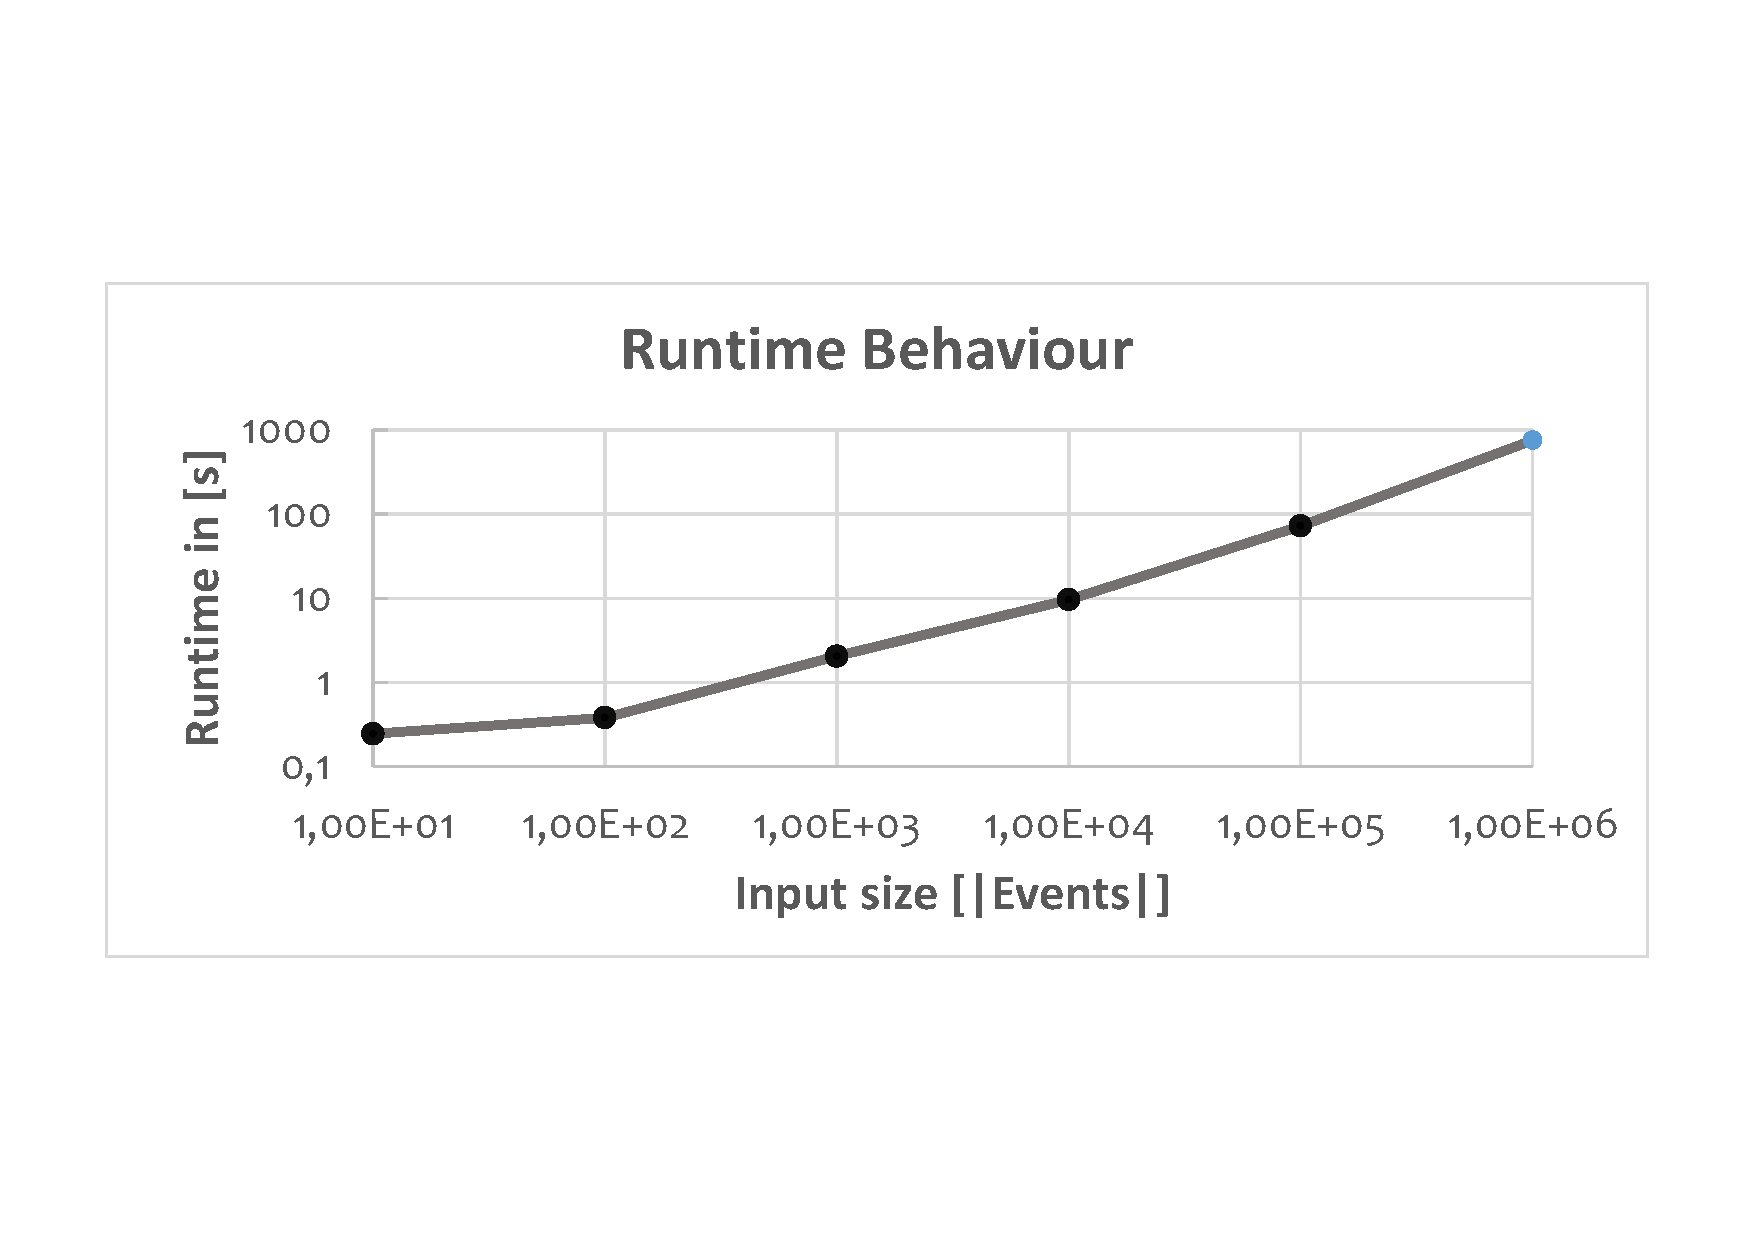
\includegraphics[trim = 0mm 40mm 0mm 40mm, clip, width=0.90\textwidth]{graphs/Runtime_Transformation}
	\caption{Runtime behaviour}
	\label{fig:eval:runtime:transformation}
\end{figure}


\section{Privacy Analysis}
\label{sec:Evaluation:privacyanalysis}

The \textit{Privacy Analysis} was extensively discussed in \autoref{ch:PrivacyConcept} (Privacy Concept) and \autoref{ch:PrivacyAnalysis} (Privacy Analysis). As described there, the privacy analysis consists of two sequential parts: \textit{Component Classification} and \textit{Deployment Analysis}. According to this tasks, the accuracy evaluation is also split. The accuracy evaluation uses the Medi-System model (\autoref{sec:eval:models:medSys}), due to its moderate complexity level, where effects like the \textit{Joining Data Stream} occurs, but the results are still traceable.

\subsection{Privacy Analysis: Accuracy Evaluation}

We will show, that the component classification categorizes components correctly, by finding \textit{joining data streams} in inter component communication. Further, we will show, that the deployment analysis finds \textit{joining data streams} on the deployment level. As a result, we demonstrate the correctness of our privacy analysis, as specified in the goal section (\autoref{sec:Introduction:goals}).

The scenarios \#1 (\autoref{eval:scenario:1}) and \#2 (\autoref{eval:scenario:1}) aim to trigger a privacy analysis. We showed in \autoref{sec:Evaluation:monitoring}, that both trigger, the TDeployment Event and the TGeoLocation Event are correctly processed and the information transformed onto the PCM model. Both trigger start the same privacy analysis and are therefore equivalent. 

\begin{figure}[h]
	\centering
	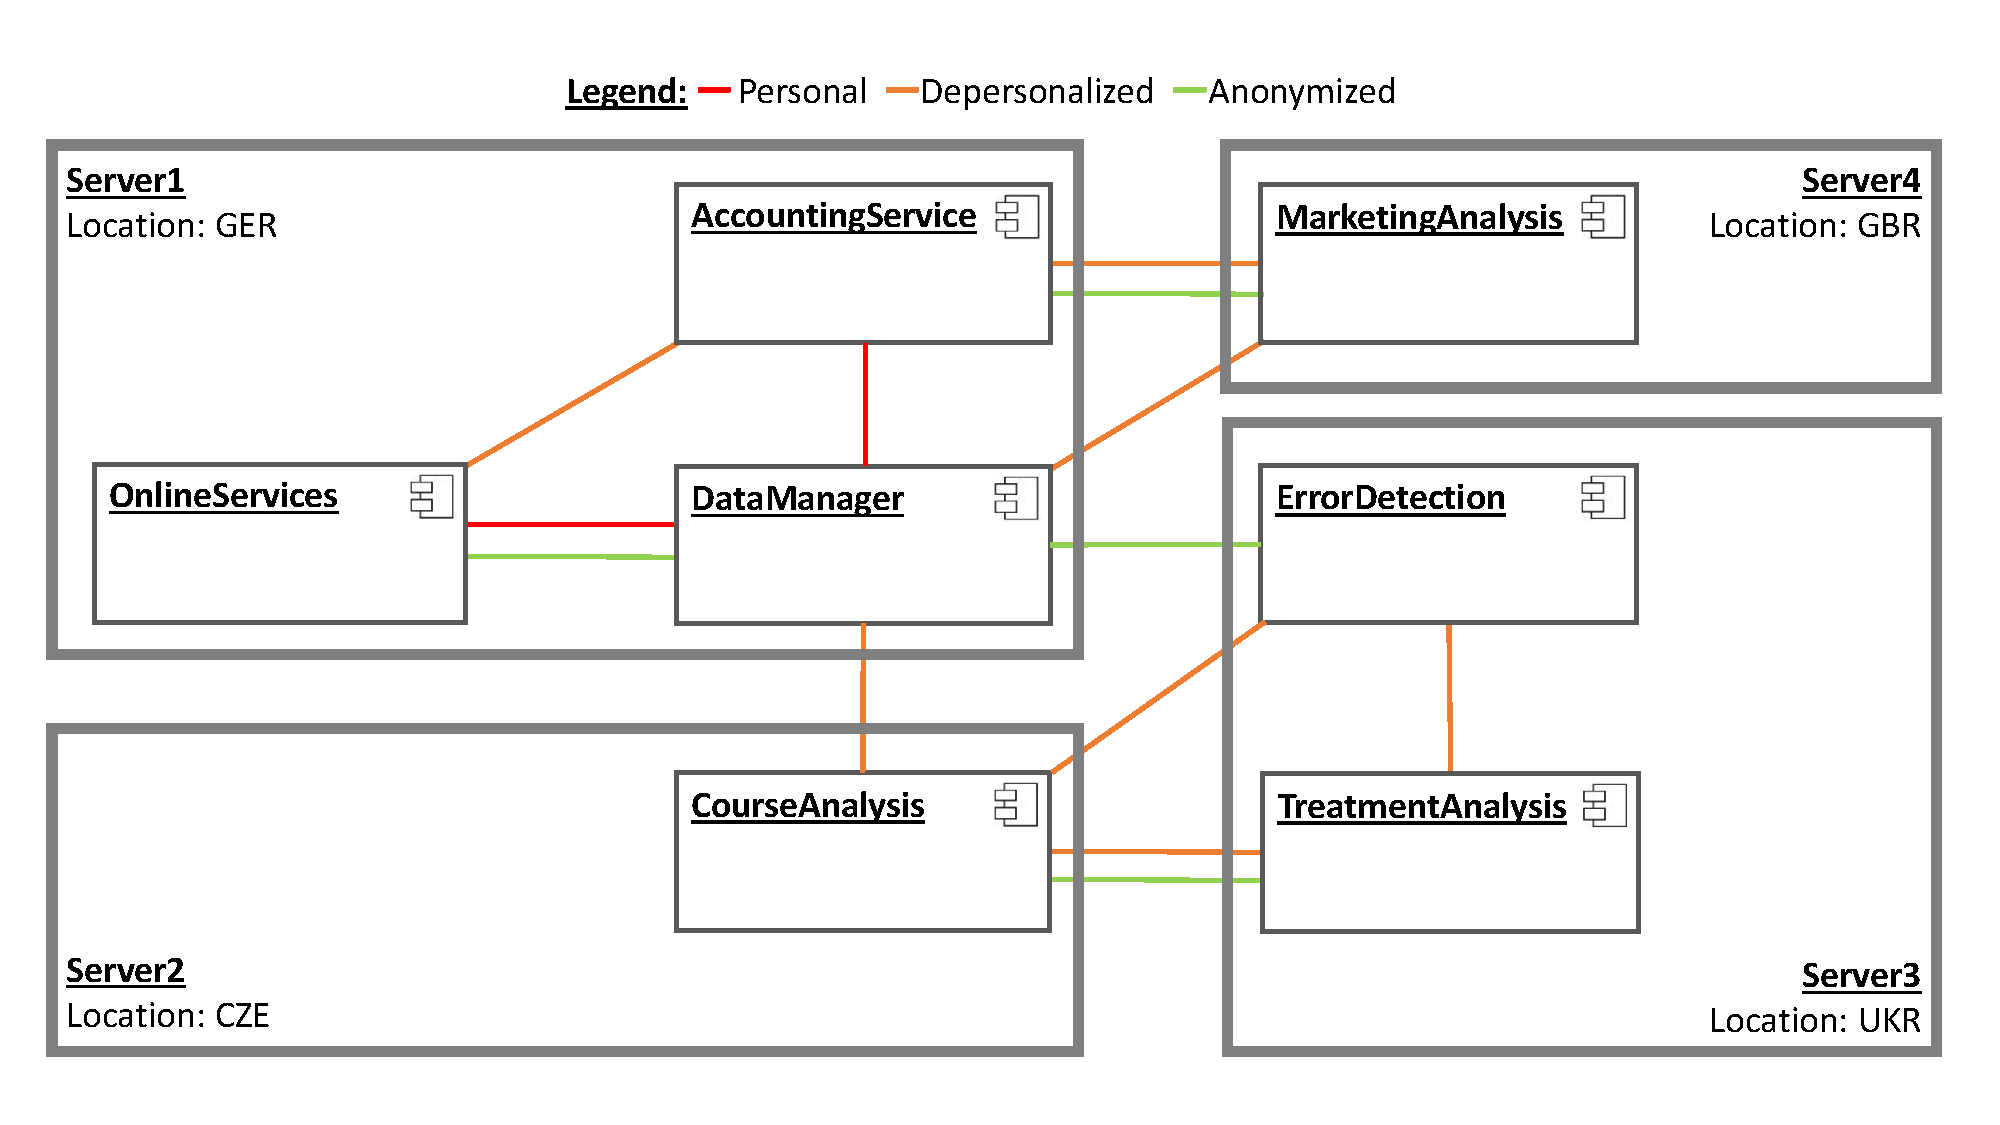
\includegraphics[trim = 0mm 10mm 0mm 10mm, clip, width=0.75\textwidth]{graphs/medSys_eval_pa_init}
	\caption{Initial system state}
	\label{fig:eval:pa:init}
\end{figure}

The initial system state is as show in \autoref{fig:eval:pa:init}. The system is privacy compliant and only the \textit{GovStatistics} component is not allocated onto a server. iObserve will trigger the pipeline by receiving a GeoLocation event, which migrates the \textit{Server2} to Belarus. We expect the initial component categorization to be equal to the most personal interface level the component has. After the \textit{Categorization Analysis} the \textit{MarketingAnalysis} component should be classified as personal, due to its two personal communication partners. The components \textit{ErrorDetection}, \textit{TreatmentAnalysis} and \textit{CourseAnalysis} data privacy level should remain unchanged, since they share a single depersonalised interface as data sources. The deployment must remain legal.

As a second trigger, we deploy the GovStatistics component onto Server2. The component must be tagged depersonalised and the deployment analysis must report a \textit{joining data stream} on Server2.

The result is \textit{unbiased}. The \autoref{fig:eval:pa:base_tag} shows the initial component categorization. \autoref{fig:eval:pa:categorized} shows the categorization analysis result. Both states fulfil the expectations. The deployment analysis reports a legal deployment.

\begin{figure}[h]
	\centering
	\begin{minipage}[b]{0.48\textwidth}		
		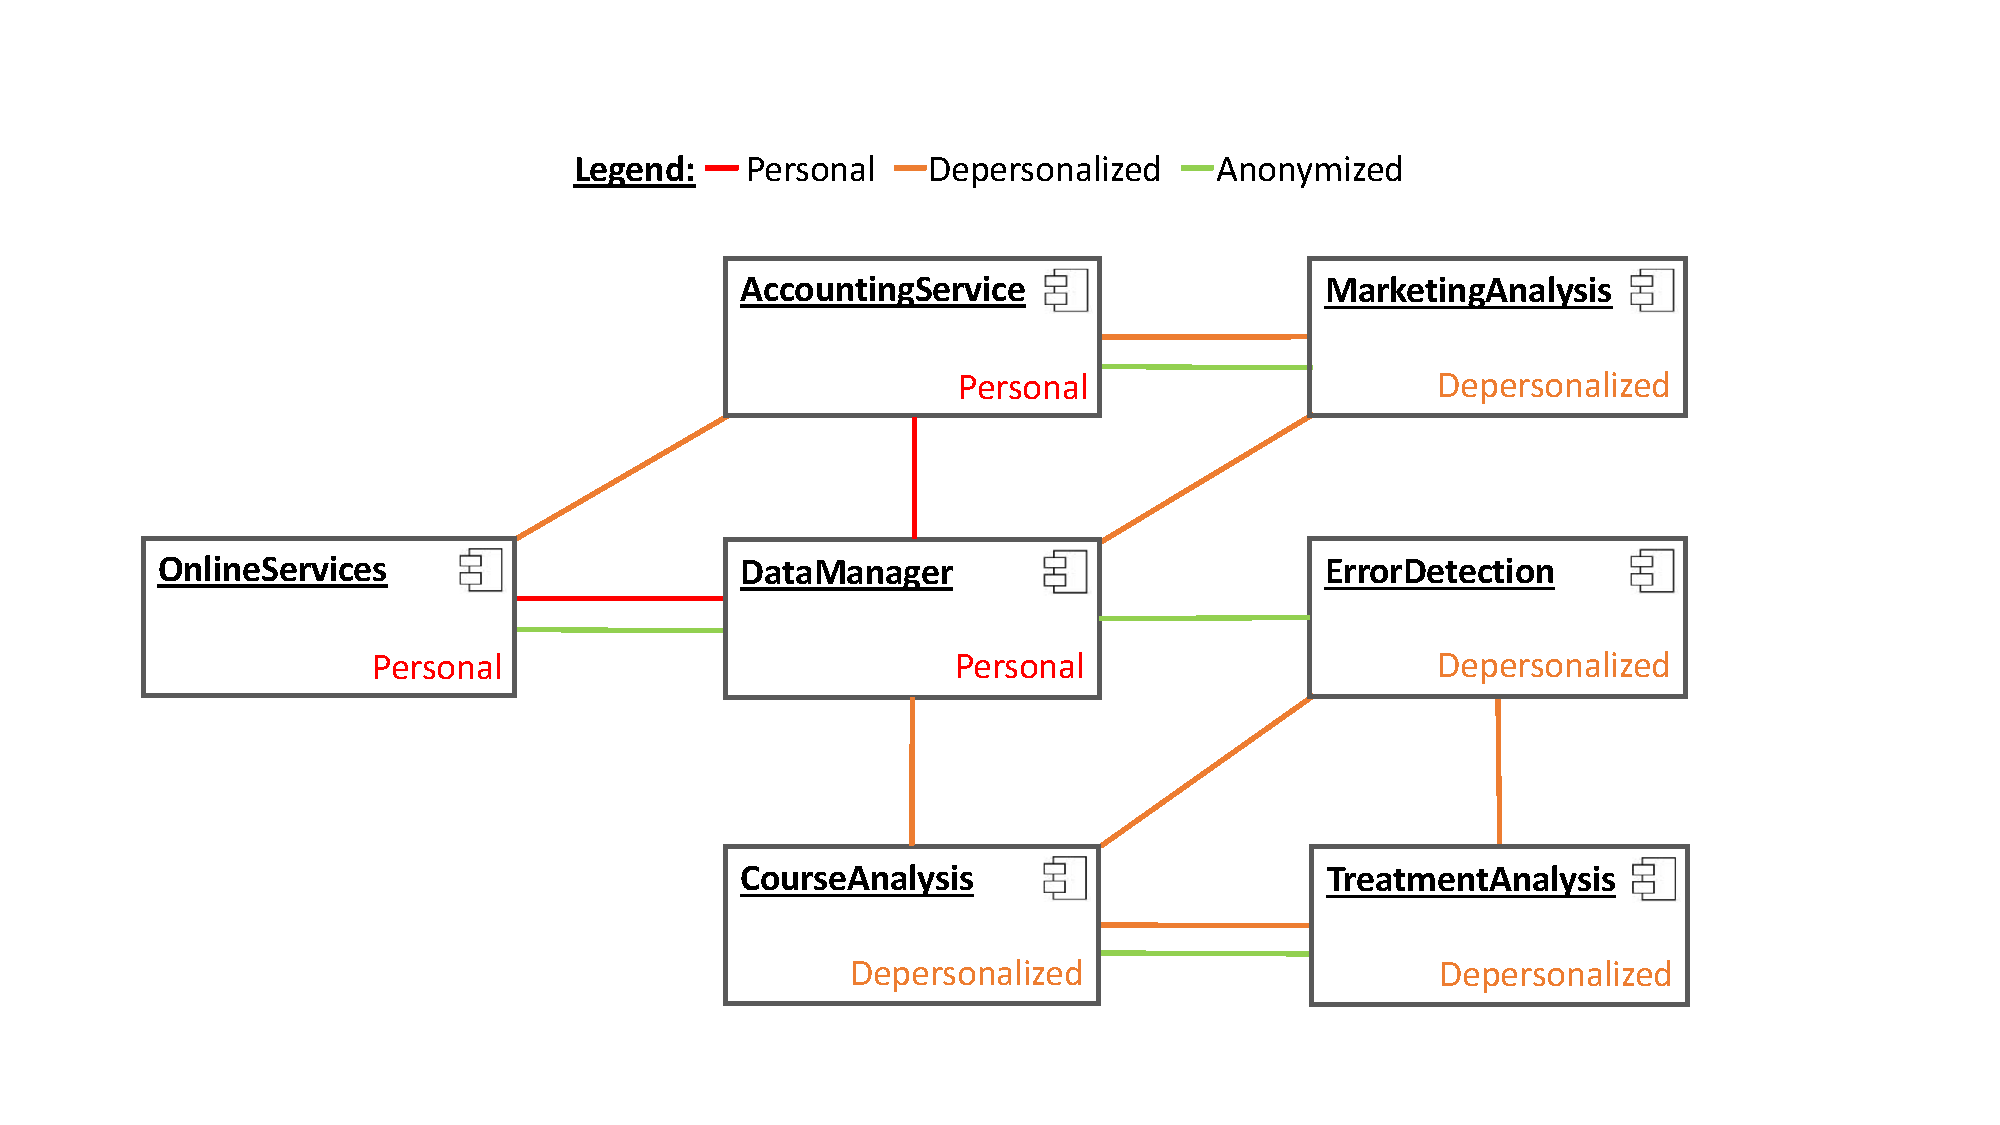
\includegraphics[trim = 20mm 10mm 40mm 10mm, clip, width=0.99\textwidth]{graphs/medSys_eval_pa_tagging_init}
		\caption{Initial categorization}
		\label{fig:eval:pa:base_tag}
	\end{minipage}
	\begin{minipage}[b]{0.48\textwidth}
		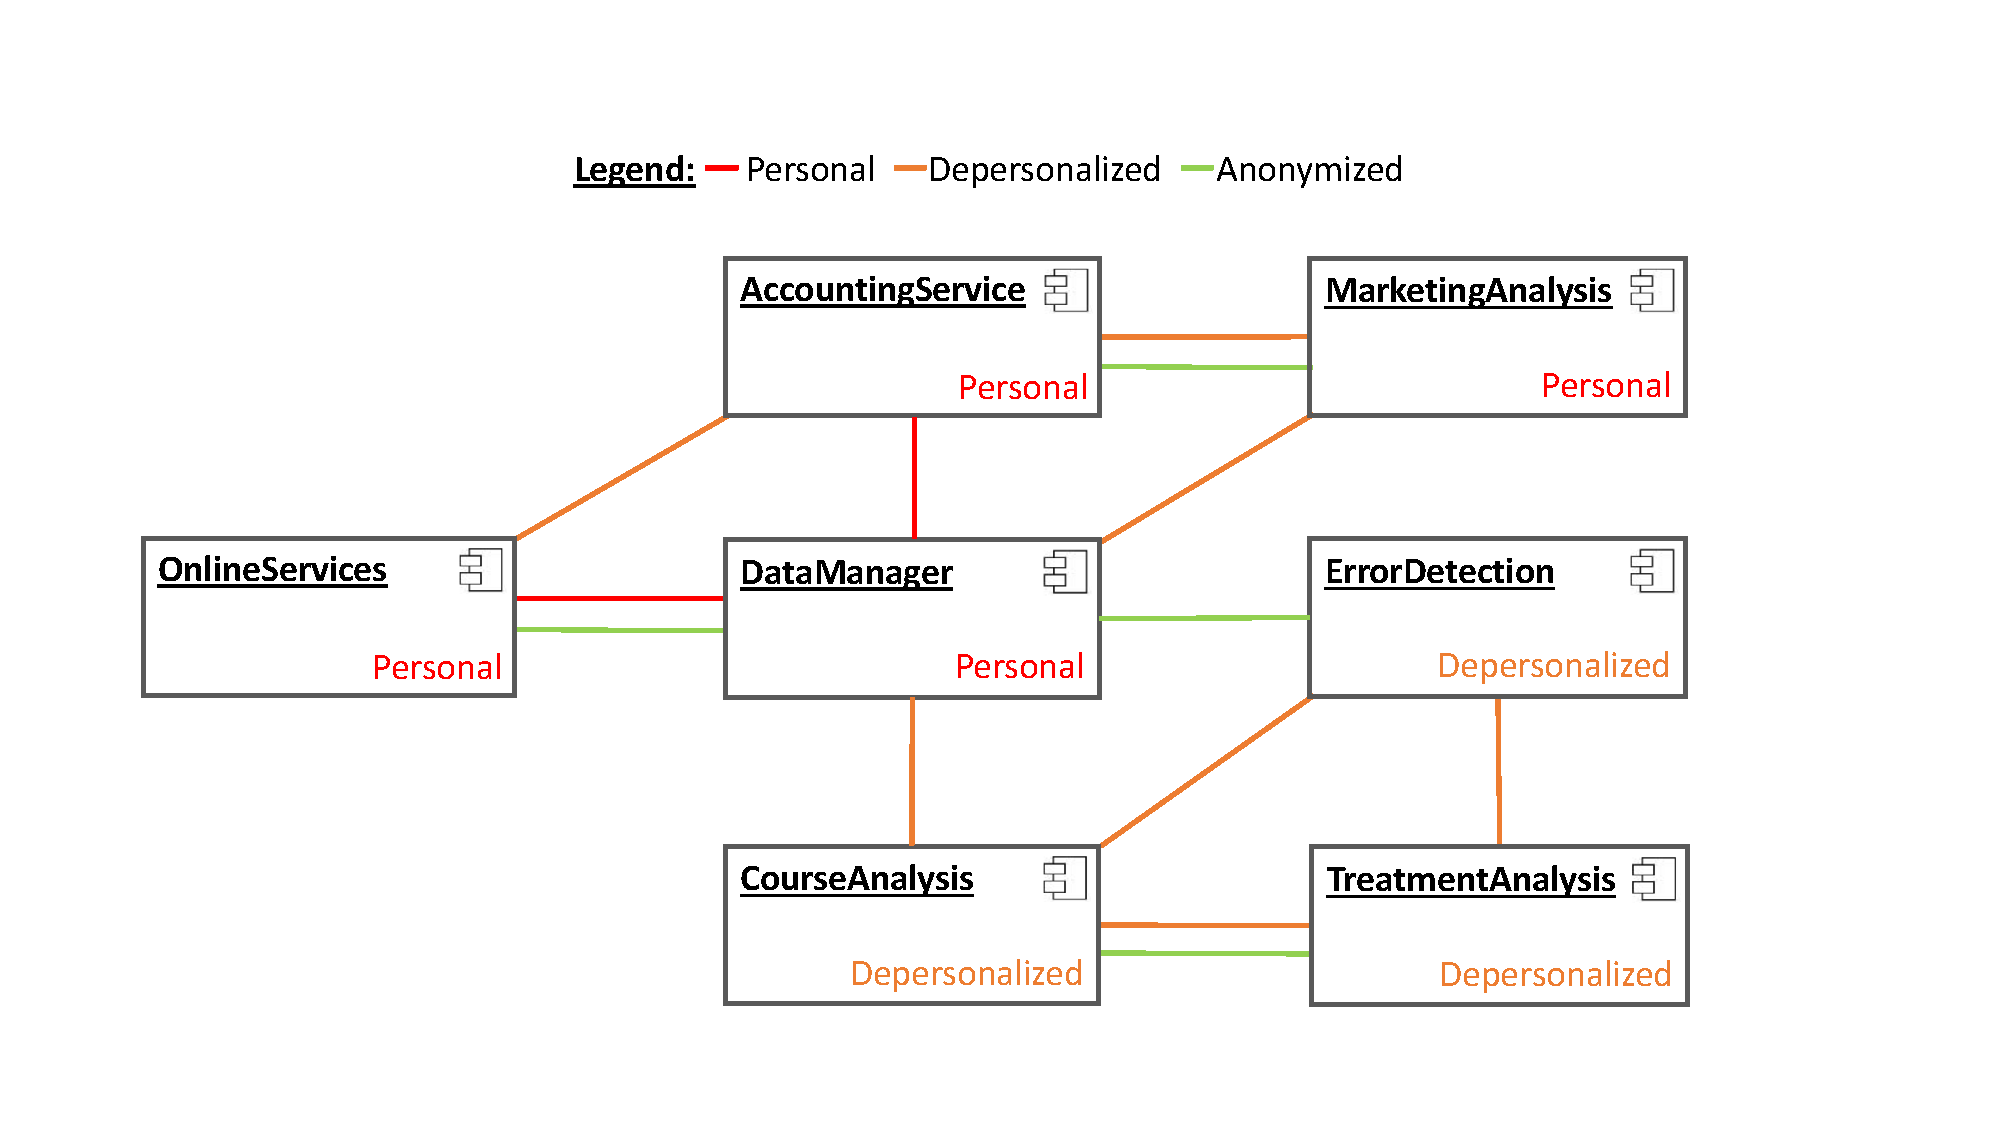
\includegraphics[trim = 20mm 10mm 40mm 10mm, clip, width=0.99\textwidth]{graphs/medSys_eval_pa_tagging_analysis}
		\caption{Categorization analysis result}
		\label{fig:eval:pa:categorized}
	\end{minipage}
\end{figure}

The second trigger, the component deployment on \textit{Server2}, reports a privacy violation. The cause is a joining data stream on Server2. This is what we provoked and expected.

\begin{figure}[h]
	\centering
	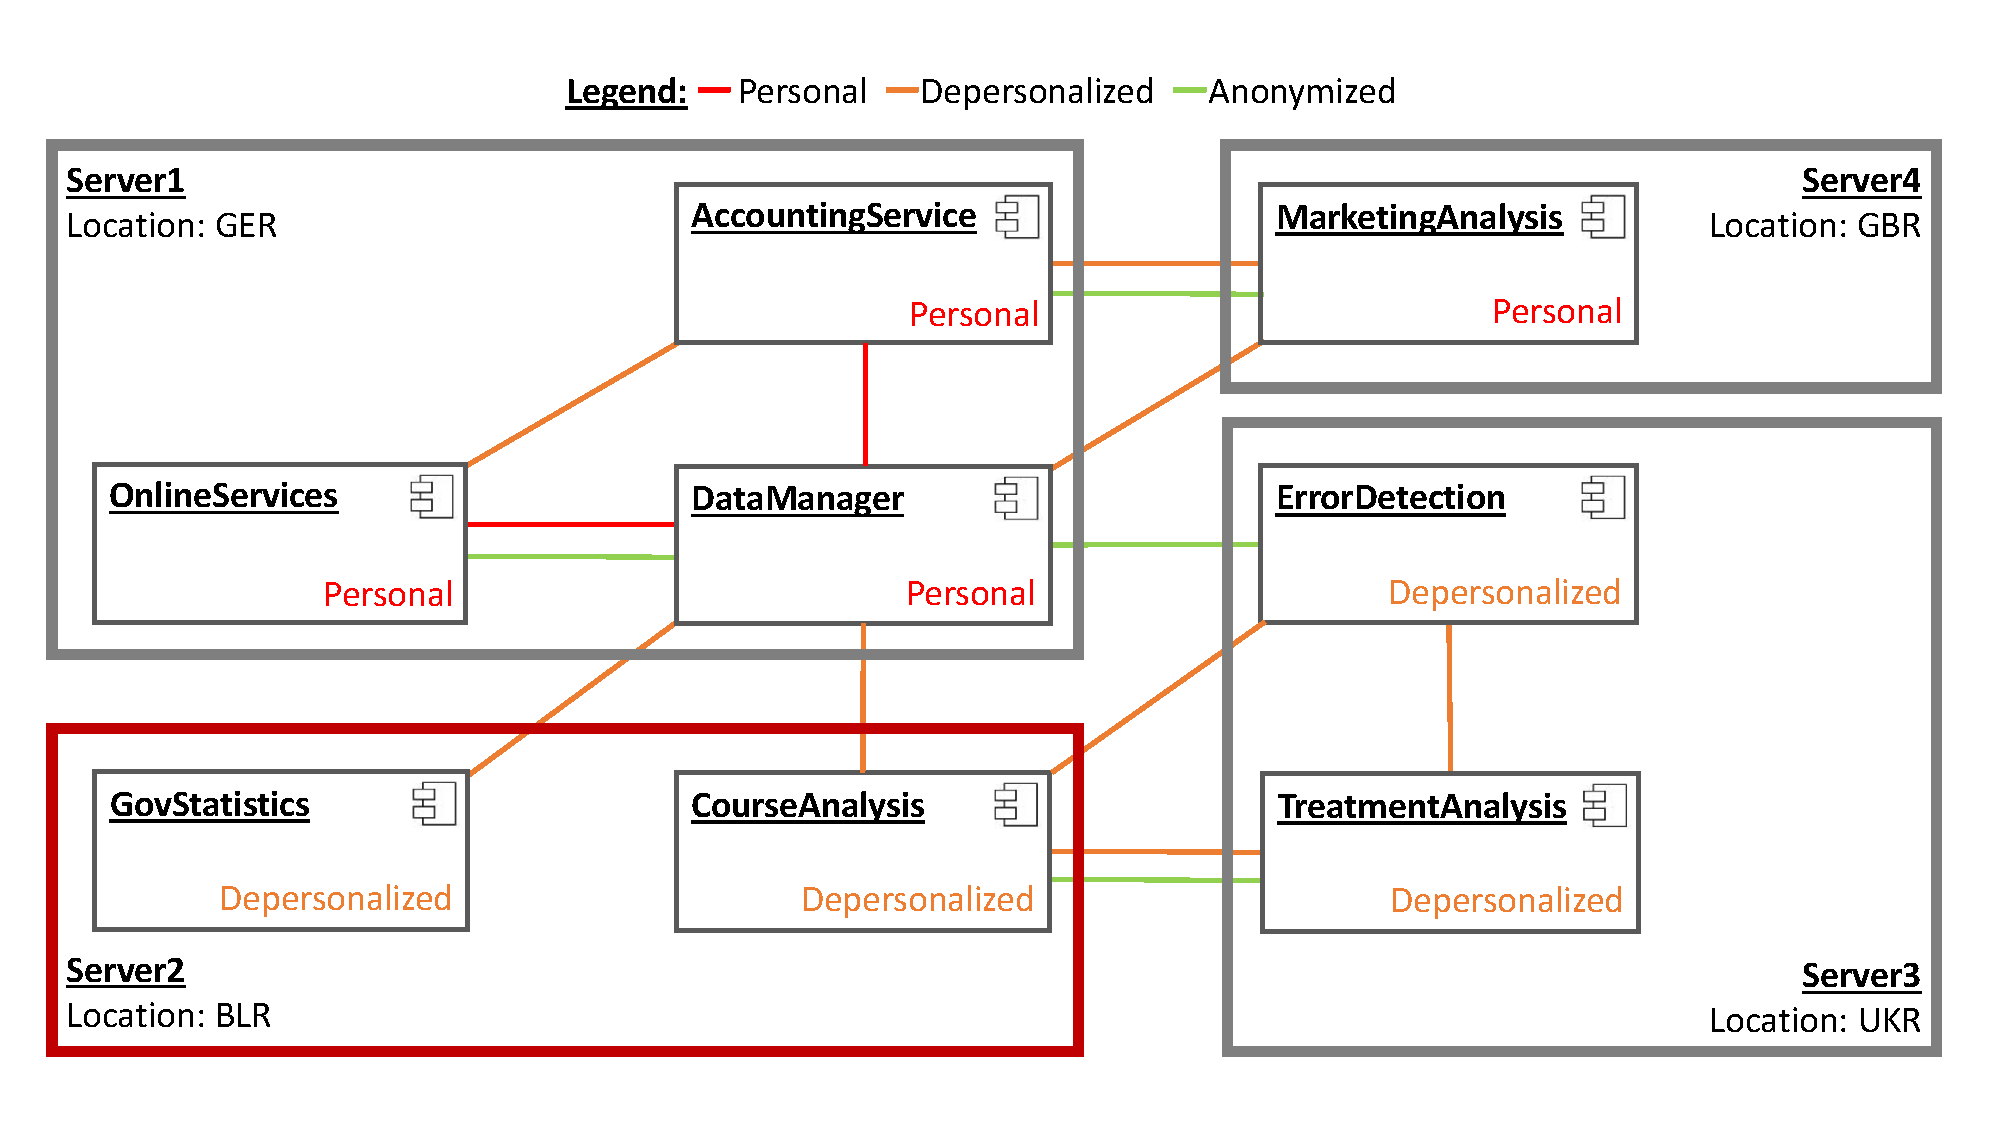
\includegraphics[trim = 0mm 10mm 0mm 10mm, clip, width=0.75\textwidth]{graphs/medSys_eval_pa_da}
	\caption{Deployment analysis result}
	\label{fig:eval:pa:depl_ana}
\end{figure}

We have shown, that the component classification algorithm and the deployment analysis works as intended, providing a privacy analysis on a architectural level (see \autoref{sec:Introduction:goals}). We didn't show every possible privacy violation, however showed the most difficult analysis work: The detection of joining data streams on component categorization and deployment analysis level. And the correct identification of a set of components, located on a server, sharing the same single depersonalised component as a data source. We will use further exemplary privacy violations in the other accuracy evaluations.

\subsection{Privacy Analysis: Scalability Evaluation}

For the scalability evaluation of the privacy analysis, we will use the generated model (\autoref{sec:Evaluation:models:generated}), since models of the intended evaluation scale are not constructable by hand. 


\section{Model Generation}
\label{sec:Evaluation:generation}

\dots

\section{Adaptation Planning}
\label{sec:Evaluation:planning}

\dots

\section{Adaptation Execution}
\label{sec:Evaluation:execution}

\dots